\subsection{Metodologia}
Sin da subito abbiamo deciso di adottare una metodologia di sviluppo \textit{Agile-Scrum}, seppur non scegliendo un vero e proprio Scrum Master.
Chi più e chi meno, a seconda dei vari sprint, ognuno ha avuto l'occasione e il modo di ricoprire tale ruolo.
In questo modo tutti hanno potuto dare il loro contributo per la riuscita del progetto, coordinando il team con l'aiuto degli strumenti a disposizione.
In accordo con tale metodologia, il lavoro è stato suddiviso in \textit{Sprint}, della durata media di una settimana e mezzo.
Allo scadere del tempo si sarebbe dovuti arrivare a sviluppare un numero minimo di funzionalità dell'applicativo.
I meeting sono stati frequenti all'inizio e ne sono stati svolti alcuni saltuariamente all'interno di ogni sprint.
Questo perché, alternandosi con un periodo di lavoro autonomo, abbiamo ritenuto necessario e producente confrontarsi anche durante gli sprint su scelte sintattiche e pattern di sviluppo tra tutti i membri del team, in modo da condividere conoscenze ed entusiasmo.

\subsection{Strumenti adottati}

\paragraph{VCS}
Si è deciso di utilizzare \textit{Git} per effettuare il versioning del codice durante lo sviluppo attraverso la piattaforma \textit{GitHub}.
L’utilizzo che ne abbiamo fatto è descritto nell'immagine di seguito:
\begin{center}
    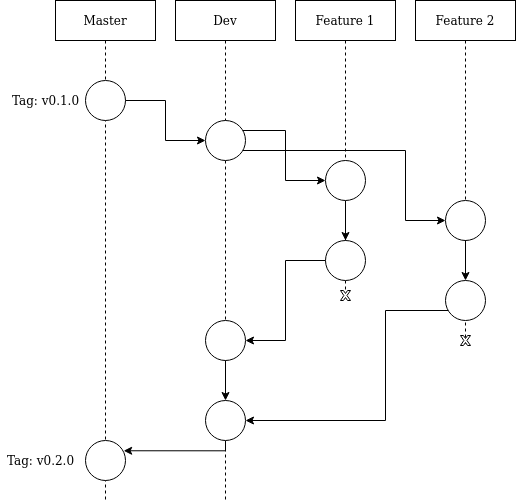
\includegraphics[scale=0.4]{git-workflow-1-1}
\end{center}
Il branch di default è sempre il \textit{master}, al quale \textit{dev} è sempre allineato.
Nel caso in cui debbano essere prodotti degli hotfix, essi vengono svolti su un branch che parte dal \textit{master} e vi ritorna subito, senza passare da \textit{dev}.
Ogni volta che si implementava una nuova funzionalità o si risolveva una fix, veniva creato una branch a parte.
Successivamente, a lavoro ultimato, veniva una creata pull request per mergiare sul branch \textit{dev}.
Ogni pull request su \textit{dev} deve essere approvata almeno da un altro membro del gruppo.
Per mergiare invece un insieme di funzionalità sviluppate e testate dal branch \textit{dev} al \textit{master}, deve sempre essere aperta una pull request, che deve essere approvata da tutti i membri del gruppo.
Questo per essere certi che tutti i membri del gruppo siano consapevoli del lavoro svolto da tutti gli altri.

\paragraph{Build Automation}
Si è deciso di usare \textit{SBT}, dato che durante il corso lo si é sempre preferito rispetto al 'cugino' \textit{Gradle} per lo svolgimento degli elaborati, nonostante il fatto che alcuni componenti del gruppo lo utilizzino in ambito aziendale.

\paragraph{Continuous Integration}
Si è deciso di usare \textit{Travis CI}.
Consisteva nell'unica soluzione freeware che i componenti del gruppo abbiano mai usato, introdotta proprio in questo corso.
Tuttavia, è stato necessario approfondire l'argomento tramite studio autonomo, dato che ciò che si era appreso a lezione é stato ritenuto insufficiente per la buona riuscita del progetto per come è stato pensato.
Ad esso é stata adattata l'esecuzione dei test necessari per verificare la correttezza del lavoro svolto e poter poi effettuare dei rilasci senza regressioni.
Tramite lo stesso servizio é stata effettuata la \textit{Continuous Delivery}, rilasciando dei pacchetti compilati su \textit{Github Releases}.

\paragraph{Bacheca}
Per avere una visione sull’andamento generale del progetto e sulle specifiche feature da svolgere o completate, abbiamo utilizzato \textit{Trello}.
\newline
Si sono realizzate delle etichette personalizzate da associare alle feature da implementare per una migliore organizzazione per ogni membro del team.
Inoltre si sono create delle colonne in cui raggruppare le feature a seconda del suo stato di sviluppo.
Alcune di queste sono:
\begin{itemize}
    \item \textit{To Do}: contiene le card associate alle features da sviluppare;
    \item \textit{Done}: contiene le card associate alle features sviluppate;
    \item \textit{Bug}: contiene le card associate alle features che presentano bug da ‘fixare’;
    \item \textit{Sprint}: contiene le card che riassumono le features da svolgere per ogni sprint.
\end{itemize}
\begin{center}
    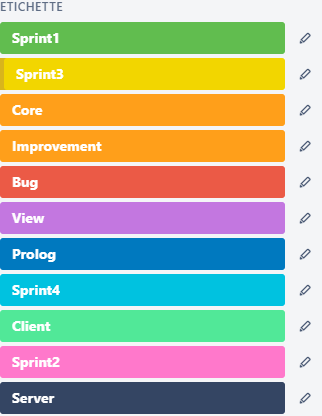
\includegraphics[scale=0.3]{etichetteTrello}
    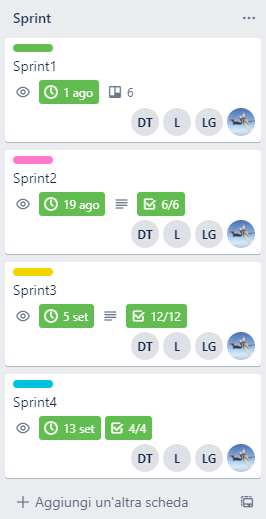
\includegraphics[scale=0.3]{SprintTrello}
\end{center}
La bacheca è possibile consultarla direttamente cliccando il link: \href{https://trello.com/b/Nk4j3Kuf/pps}{Trello}.

\paragraph{Test}
Durante il progetto si è data importanza anche allo sviluppo dei test.
In particolare ogni membro del team, ha testato tutte le features da lui sviluppate creandone ad-hoc utilizzando l'approccio più consono.
Ogni sviluppatore prima di poter eseguire una pull request della propria features, doveva controllare che i test eseguiti passassero non solo in locale ma anche sul server di CI.
Lo sviluppo dei test è stato di aiuto soprattutto negli Sprint 3 e 4 poiché ci hanno permesso di individuare e di risolvere i bug più velocemente.

\newpage